\documentclass{beamer}
%\documentclass[11pt, handout]{beamer}

\usepackage{graphicx}
\usepackage{xspace}
\usepackage{tikz}
\usepackage{circuitikz}
\usepackage{hyperref}
\usepackage{adjustbox} 
\usepackage{protocolj}
\usepackage{multirow}
\usepackage{longtable,booktabs,setspace} 
\usetikzlibrary{shapes.geometric, arrows}

%% Alex L's macros 
%% taken and co-opted from a variety of sources
%
%% generic commands
%\newcommand{\NN}{\mathbb{N}}
%\newcommand{\RR}{\mathbb{R}}
%\newcommand{\compindist}{\approx_C}
%
%% definition counter
%\newcounter{defcounter}
%\setcounter{defcounter}{0}
%\newenvironment{definition}{\medskip\noindent\refstepcounter{defcounter}{\bf Definition \thedefcounter}\hspace*{2pt}}{\hspace*{\fill}\nopagebreak[4]$\diamondsuit$\medskip}  
%
%% block quote
%\newenvironment{blockquote}{%
%  \par%
%  \medskip
%  \leftskip=4em\rightskip=2em%
%  \noindent\ignorespaces}{%
%  \par\medskip}
%
%% Author Macros -- colors: red, magenta, blue, orange
%\newcounter{al}
%\newcommand{\al}[1]{\textcolor{blue}{\{AL-\arabic{al}: #1\}}\addtocounter{al}{1}}
%\newcounter{cat}
%\newcommand{\cat}[1]{\textcolor{magenta}{\{CAT-\arabic{cat}: #1\}}\addtocounter{cat}{1}}
%\newcommand{\ignore}[1]{}
%
%% From CompGC paper
%%\renewcommand{\sim}{S}
%%\newcommand{\Input}{\ensuremath{\textsf{Input}}\xspace}
%%\newcommand{\Output}{\ensuremath{\textsf{Output}}\xspace}
%%\newcommand{\Inputs}{\ensuremath{\textsf{Inputs}}\xspace}
%%\newcommand{\Outputs}{\ensuremath{\textsf{Outputs}}\xspace}
%%\newcommand{\Components}{\ensuremath{\textsf{Components}}\xspace}
%
%\newcommand{\Gates}{\text{Gates}}
\newcommand{\C}{\sf {C}}
\newcommand{\GC}{\sf {GC}}
%\newcommand{\AllInputLabels}{\sf {AllInputLabels}}
%\newcommand{\InputLabels}{\sf {InputLabels}}
%\newcommand{\InputWires}{\text{InputWires}}
%\newcommand{\OutputWires}{\text{OutputWires}}
%\newcommand{\Wires}{\text{Wires}}
%\newcommand{\A}{\mathcal{A}}
%\newcommand{\OT}{\textsf{OT}} % or mathsf
\newcommand{\Enc}{\textsf{Enc}} % or mathsf
\newcommand{\Dec}{\textsf{Dec}}
\newcommand{\Gen}{\textsf{Gen}}
\newcommand{\EncInv}{\Enc^{-1}}
\newcommand{\EncDKC}{\textsf{EncDKC}}
\newcommand{\DecDKC}{\textsf{DecDKC}}
\newcommand{\EncDKCInv}{\EncDKC^{-1}}
%\newcommand{\compIndist}{\approx_D}
%\newcommand{\outputrv}{{\sf output}}
%\newcommand{\viewrv}{{\sf view}}
\newcommand{\CompGC}{\textsf{CompGC}\xspace}
%\newcommand{\JustGarble}{\textsf{JustGarble}\xspace}
%\newcommand{\Naive}{\textsf{Naive}\xspace}
%\newcommand{\scmc}{SCMC\xspace} % Single Communication Multiple Connnection


\newcommand\Wider[2][3em]{%
\makebox[\linewidth][c]{%
  \begin{minipage}{\dimexpr\textwidth+#1\relax}
  \raggedright#2
  \end{minipage}%
  }%
}

\renewcommand<>{\item}[1]{\only#2{\beameroriginal{\item}{#1}}}
    \mode<presentation> {
        \usetheme{default}
        \usecolortheme{seahorse}
        \setbeamertemplate{footline}[page number] 
        \setbeamertemplate{navigation symbols}{} 
    }

    \title[Short title]{Implementing Component-Based Garbled Circuits\\
    } 
    \author{Alex Ledger} 
    \institute[Reed College]{
        Reed College \\ 
    }
    \date{\today}

    \begin{document}

        \begin{frame}
            \titlepage
        \end{frame}

        \begin{frame}
            \frametitle{Security of Encryption}
            An encryption scheme is secure under a chosen-plaintext attack if for all probabilistic polynomial-time adversaries $A$, there exists a negligible function $\mu$ such that
            \begin{align*}
                Pr[E_{\A, \Pi}(n) = 1] \leq \frac{1}{2} + \mu(n)
            \end{align*}
            where $E$ is the following experiment:
            \begin{enumerate}
                \item Generate key $k$ by running $\Gen(1^n)$. 
                \item The adversary $\A$ is given $1^n$ and oracle access to $\Enc_k$, and outputs a pair of messages $m_0$ and $m_1$ of the same length.
                \item A uniform bit $b \samples \{0,1\}$ is sampled uniformly at random, and then ciphertext $c \gets \Enc_k(m_b)$ is computed and given to $\A$.
                \item Then $\A$ continues to have oracle access to $\Enc_k$, and outputs a bit $b'$. 
                \item The output of the experiment is defined to be $1$ if $b' = b$ and $0$ otherwise. If at any point $\A$ encrypts $m_0$ or $m_1$ with their encryption oracle, the output is $0$. $1$ indicates that the adversary wins, and $0$ indicates that the adversary loses.
            \end{enumerate}
        \end{frame}

        \begin{frame}
            \frametitle{Computational Indistinguishability}
            Intuition: 
            \begin{itemize}
                \item Let $\mathcal{X}$ and $\mathcal{Y}$ be distribution ensembles.
                \item Give an adversary one of the distribution ensembles.
                \item Can the adversary sample from the distribution a polynomial number of times to determine which distribution they were given?
            \end{itemize}

            Formal Definition:
            \begin{itemize}
                \item Let $\mathcal{X} = \{X_n\}_{n \in \NN}$ and $\mathcal{Y} = \{Y_n\}_{n \in \NN}$ be distribution ensembles.
                \item Then $\mathcal{X}$ and $\mathcal{Y}$ are computationally indistinguishable, denoted $\mathcal{X} \compindist \mathcal{Y}$, if for all probabilistic polynomial-time algorithms $D$, there exists a negligible function $\mu$ such that:
                    \begin{align*}
                        |Pr_{x \gets X_n} [D(1^n, x) = 1] - Pr_{y \gets Y_n} [D(1^n, y) = 1]| < \mu(n)
                    \end{align*}
            \end{itemize}
        \end{frame}

        \begin{frame}
            \frametitle{Oblivious Transfer 2}
            \begin{figure}
                \centering
                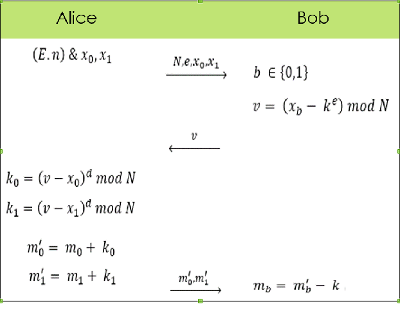
\includegraphics[scale=0.5]{images/ot_details}
                % https://www.codechef.com/problems/OBLIVI
            \end{figure}
            RSA-based oblivious transfer
        \end{frame}

        \begin{frame}
            \frametitle{Security of 2PC (Overview)}
            \begin{figure}
                \centering
                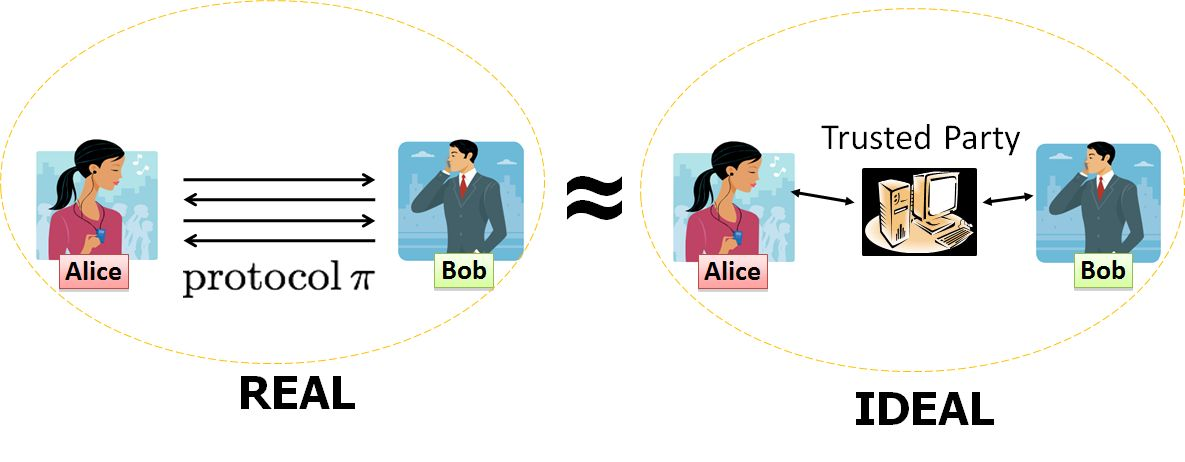
\includegraphics[scale=0.25]{images/security}
            \end{figure}
        \end{frame}

        \begin{frame}
            \frametitle{Security of 2PC (Ideal World)}
                Define the following:
                \begin{align*}
                    \{\sim_A(x, f(x,y)\}_{x \in \{0,1\}^*} \\
                    \{\sim_B(y, f(x,y)\}_{y \in \{0,1\}^*}
                \end{align*}
                \begin{align*}
                    & \{\viewrv_A(x, y)\}_{x, y \in \{0,1\}^*} \\
                    & \{\viewrv_B(x, y)\}_{x, y \in \{0,1\}^*} 
                \end{align*}
                \begin{align*}
                    output^{\Pi}_i(n,x,y)
                \end{align*}
                Then $\Pi$ is secure if:
                \begin{align*}
                    & \{(S_A(x, f_A(x,y)), f(x,y))\}_{x,y} \compindist \{(\viewrv^{\Pi}_A(x,y), \outputrv^{\Pi}(x,y)) \}_{x,y} \\
                    & \{(S_B(x, f_B(x,y)), f(x,y))\}_{x,y} \compindist \{(\viewrv^{\Pi}_B(x,y), \outputrv^{\Pi}(x,y)) \}_{x,y} 
                \end{align*}
        \end{frame}

        \begin{frame}
            \frametitle{Garbled Circuits}
            \begin{enumerate}
                \item Alice assigns wire labels
                \item Alice make garbled tables
                    \begin{itemize}
                        \item Alice permutes rows
                    \end{itemize}
                \item Alice sends garbled tables to Bob
                \item Alice sends input wire labels to Bob
                    \begin{itemize}
                        \item Some are sent via OT
                        \item Others are simply sent
                    \end{itemize}
                \item Bob trial decrypts each row of garbled table with input wire labels
                \item Bob acquires output wire label
                \item Bob uses output wire label in subsequent gates
                \item Bob eventually acquires output wire labels
            \end{enumerate}
        \end{frame}

        \begin{frame}
            \frametitle{Improvements to Garbled Circuits}
            \begin{table}[t]
    \centering
    \renewcommand{\arraystretch}{1.2}
    \normalsize
    \begin{adjustbox}{width=1\textwidth}
        \begin{tabular}{|p{5cm}|c|c|c|c|c|c|}
            \hline
            \multirow{2}{5cm}{\centering \textbf{Garbled Circuit Improvement}} & 
            \multicolumn{2}{c|}{\textbf{Table Size (x$\lambda$)}} & 
            \multicolumn{2}{c|}{\textbf{Garble Cost}} & 
            \multicolumn{2}{c|}{\textbf{Eval Cost}} \\
            \cline{2-7}
            & \textbf{XOR} & \textbf{AND} & \textbf{XOR} & \textbf{AND}  & \textbf{XOR} & \textbf{AND} \\
            \hline
            Classical & 4 & 4 & 4 & 4 & 4 & 4 \\ \hline
            Point and Permute & 4 & 4 & 4 & 4 & 1 & 1 \\ \hline
            GRR3 & 3 & 3 & 4 & 4  & 1 & 1 \\ \hline
            Free XOR & 0 & 3 & 0 & 4 & 0 & 1  \\ \hline
            GRR2  & 2 & 2 & 4 & 4 & 1 & 1  \\ \hline
            FleXOR & \{0,1,2\} & 2 & \{0,2,4\} & 4 & \{0,1,2\} & 1  \\ \hline
            Half Gates & 2 & 0 & 2 & 0 & 0 & 2  \\ \hline
        \end{tabular}
    \end{adjustbox}
    \caption{Table size is number of ciphertexts. Garble cost is number of encryptions the garbler performs. Eval cost is number of decryptions the evaluator performs.}
\end{table}



        \end{frame}

        \begin{frame}
            \frametitle{Point and Permute}
            All examples use an AND gate with input wires $W_i$ and $W_j$ and output wire $W_k$.
            \begin{table}
                \label{tbl:point-and-permute}
                \centering
                \begin{tabular}{|c|c|}
                    \hline
                    Select Bit & Wire Label \\
                    \hline
                    0 & $W_i^0$ \\
                    1 & $W_i^1$ \\
                    1 & $W_j^0$ \\
                    0 & $W_j^1$ \\
                    \hline
                \end{tabular}
                \qquad
                \begin{tabular}{|c|c|}
                    \hline
                    Select Bits & Encryption \\
                    \hline
                    (0,0) & $\Enc_{W_i^0, W_j^1}(W_k^0)$ \\
                    (0,1) & $\Enc_{W_i^0, W_j^0}(W_k^0)$ \\
                    (1,0) & $\Enc_{W_i^1, W_j^1}(W_k^1)$ \\
                    (1,1) & $\Enc_{W_i^1, W_j^0}(W_k^0)$ \\
                    \hline
                \end{tabular}
                \caption[Garbled table with point and permute]{Garbled AND gate for Point and Permute}
            \end{table}


        \end{frame}

        \begin{frame}
            \frametitle{Garbled Row Reduction 3}
            \begin{table}
                \centering
                \begin{tabular}{|c|c|}
                    \hline
                    Select Bit & Wire Label \\
                    \hline
                    0 & $W_i^0$ \\
                    1 & $W_i^1$ \\
                    1 & $W_j^0$ \\
                    0 & $W_j^1$ \\
                    \hline
                \end{tabular}
                \qquad
                \begin{tabular}{|c|c|}
                    \hline
                    Select Bits & Encryption \\
                    \hline
                    (0,1) & $\Enc_{W_i^0, W_j^0}(W_k^0)$ \\
                    (1,0) & $\Enc_{W_i^1, W_j^1}(W_k^1)$ \\
                    (1,1) & $\Enc_{W_i^1, W_j^0}(W_k^0)$ \\
                    \hline
                \end{tabular}
                \qquad
                \begin{tabular}{|c|}
                    \hline
                    $W_k^0 \gets \Enc_{W_i^0, W_j^1}^{-1}(0^n)$ \\
                    $W_k^1 \samples \{0,1\}^n$ \\
                    \hline
                \end{tabular}
                \label{tbl:grr3}
            \end{table}
        \end{frame}

        \begin{frame}
            \frametitle{Free XOR}
            \begin{itemize}
                    \small
                \item Let $\Delta \gets \{0,1\}^n$ be fixed globally in a circuit.
                \item For each input wire:
                    \begin{itemize}
                        \item Sample $W_i^0$ randomly.
                        \item Set $W_i^1 \gets W_i^0 \oplus \Delta$.
                    \end{itemize}
                \item For each output wire of a gate $W_k$
                    \begin{itemize}
                        \item Set $W_k^0 \gets W_i^0 \oplus W_j^0$.
                        \item Set $W_k^1 \gets W_k^0 \oplus \Delta$.
                    \end{itemize}
                \item Bob \textit{evaluates} the XOR gate by XORing the two input labels.
                    \begin{align*}
                        (A \oplus a\Delta) \oplus (B \oplus b\Delta) = A \oplus B \oplus (a \oplus b)\Delta
                    \end{align*}
                \item So XOR gates do not require a garbled table, aka they're Free.
            \end{itemize}
        \end{frame}

        \begin{frame}
            \frametitle{OT-preprocessing}
            \begin{figure}
                \centering
                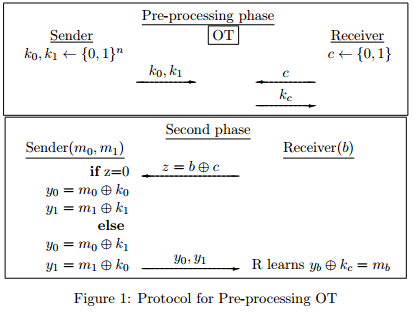
\includegraphics[scale=0.5]{images/ot-preproc}
            \end{figure}
            Source: Katz lecture notes
            % http://drona.csa.iisc.ernet.in/~arpita/StudyGroupOT15/JoKaLec3.pdf 
        \end{frame}

        \begin{frame}
            \frametitle{Motivating Component-Based GCs}
            \begin{itemize}
                \item Split protocols into offline/online 
                    \begin{itemize}
                        \item Garble and send circuit in offline phase.
                        \item Determine inputs during online phase, evaluate.
                    \end{itemize}
                \item Problem: function chosen ahead of time - no flexiblity
            \end{itemize}
        \end{frame}

        \begin{frame}
            \frametitle{Details of Component-Based Garbled Circuits (1)}
                \begin{figure}
                    %!TEX root = thesis.tex


\begin{figure}
    \centering
    \scalebox{0.8}{
    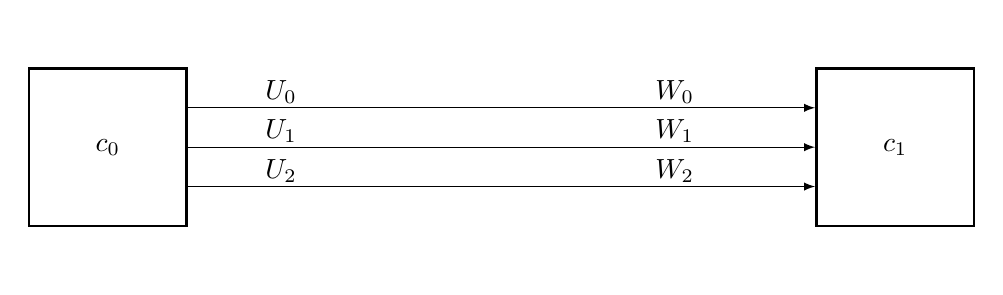
\begin{tikzpicture}
        [
            square/.style = {draw, shape=rectangle, minimum height=2cm, minimum width=2cm, node distance=2cm, line width=1pt},
            empty/.style = {draw, shape=rectangle, minimum height=2cm, minimum width=2cm, node distance=2cm, line width=1pt, draw=white},
        ]

        \node[empty] (0a) at (0,0.5)     {};
        \node[empty] (0b) at (0,-0.5)     {};
        \node[square] (0c) at (0,0)     {$c_0$};

        \node[empty] (1a) at (10cm,0.5)   {};
        \node[empty] (1b) at (10cm,-0.5)   {};
        \node[square] (1c) at (10cm,0)   {$c_1$};

        \node (x0) at (2.2cm,0.7) {$U_0$};
        \node (y0) at (2.2cm,-0.3) {$U_2$};
        \node (z0) at (2.2cm,0.2) {$U_1$};

        \node (x1) at (7.2cm,0.7) {$W_0$};
        \node (y1) at (7.2cm,-0.3) {$W_2$};
        \node (z1) at (7.2cm,0.2) {$W_1$};

        \draw [-latex] (0a.east) -- (1a.west);
        \draw [-latex] (0b.east) -- (1b.west);
        \draw [-latex] (0c.east) -- (1c.west);
    \end{tikzpicture}

}
\end{figure}

                \end{figure}
        \end{frame}

        \begin{frame}
            \frametitle{Details of Component-Based GCs (2)}
                \begin{figure}
                    %!TEX root = thesis.tex

\begin{figure}
\centering
\scalebox{0.8}{
    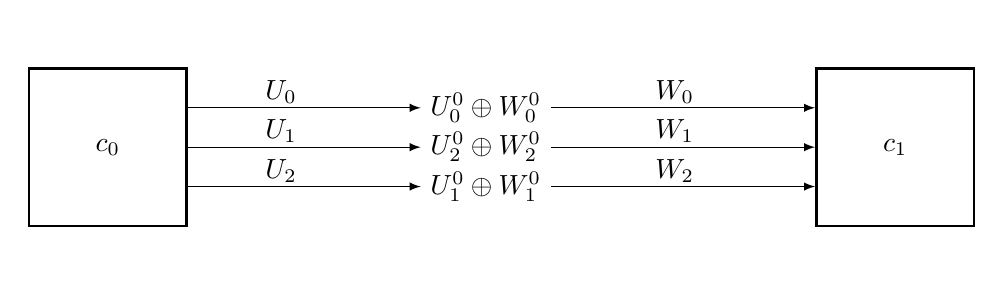
\begin{tikzpicture}
        [
            square/.style = {draw, shape=rectangle, minimum height=2cm, minimum width=2cm, node distance=2cm, line width=1pt},
            empty/.style = {draw, shape=rectangle, minimum height=2cm, minimum width=2cm, node distance=2cm, line width=1pt, draw=white},
        ]

        \node[empty] (0a) at (0,0.5)     {};
        \node[empty] (0b) at (0,-0.5)     {};
        \node[square] (0c) at (0,0)     {$c_0$};

        \node[color=black] (mida) at (4.8cm,0.5)   {$U_0^0\oplus W_0^0$};
        \node[color=black] (midb) at (4.8cm,-0.5)  {$U_1^0 \oplus W_1^0$}; 
        \node[color=black] (midc) at (4.8cm,0)     {$U_2^0 \oplus W_2^0$};

        \node[empty] (1a) at (10cm,0.5)   {};
        \node[empty] (1b) at (10cm,-0.5)   {};
        \node[square] (1c) at (10cm,0)   {$c_1$};

        \node (x0) at (2.2cm,0.7) {$U_0$};
        \node (y0) at (2.2cm,-0.3) {$U_2$};
        \node (z0) at (2.2cm,0.2) {$U_1$};

        \node (x1) at (7.2cm,0.7) {$W_0$};
        \node (y1) at (7.2cm,-0.3) {$W_2$};
        \node (z1) at (7.2cm,0.2) {$W_1$};

        \draw [-latex] (0a.east) -- (mida.west);
        \draw [-latex] (0b.east) -- (midb.west);
        \draw [-latex] (0c.east) -- (midc.west);

        \draw [-latex] (mida.east) -- (1a.west);
        \draw [-latex] (midb.east) -- (1b.west);
        \draw [-latex] (midc.east) -- (1c.west);
    \end{tikzpicture}
}
\end{figure}


                \end{figure}
        \end{frame}

        \begin{frame}
            \frametitle{Single Communcation Multiple Connections SCMC}
            % http://tex.stackexchange.com/questions/201071/how-do-i-make-tikz-circular-arrowheads-concentric-to-the-point-they-connect
            \begin{itemize}
                \item For each piece of data, sample a label $A$.
                \item Set $i$th wire label of data to $A \oplus H(i)$.
                \item Where $H$ is a hash function
            \end{itemize}

            \begin{figure}
                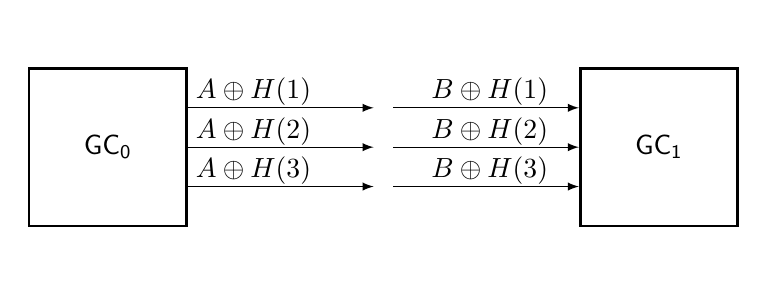
\begin{tikzpicture}
                    [
                        square/.style = {draw, shape=rectangle, minimum height=2cm, minimum width=2cm, node distance=2cm, line width=1pt},
                        empty/.style = {draw, shape=rectangle, minimum height=2cm, minimum width=2cm, node distance=2cm, line width=1pt, draw=white},
                    ]

                    \node[empty] (0a) at (0,0.5)     {};
                    \node[empty] (0b) at (0,-0.5)     {};
                    \node[square] (0c) at (0,0)     {$\GC_0$};

                    \node (mida) at (3.5cm,0.5)     {};
                    \node (midb) at (3.5cm,-0.5)     {};
                    \node (midc) at (3.5cm,0)     {};

                    \node[empty] (1a) at (7cm,0.5)   {};
                    \node[empty] (1b) at (7cm,-0.5)   {};
                    \node[square] (1c) at (7cm,0)   {$\GC_1$};

                    \node (x0) at (1.85cm,0.7) {$A \oplus H(1)$};
                    \node (y0) at (1.85cm,-0.3) {$A \oplus H(3)$};
                    \node (z0) at (1.85cm,0.2) {$A \oplus H(2)$};

                    \node (x1) at (4.85cm,0.7) {$B \oplus H(1)$};
                    \node (y1) at (4.85cm,-0.3) {$B \oplus H(3)$};
                    \node (z1) at (4.85cm,0.2) {$B \oplus H(2)$};

                    \draw [-latex] (0a.east) -- (mida);
                    \draw [-latex] (0b.east) -- (midb);
                    \draw [-latex] (0c.east) -- (midc);

                    \draw [-latex] (mida) -- (1a.west);
                    \draw [-latex] (midb) -- (1b.west);
                    \draw [-latex] (midc) -- (1c.west);
                \end{tikzpicture}
            \end{figure}
            \begin{itemize}
                \item Technically, we set the links to $A \oplus H (T \oplus (i || b))$
            \end{itemize}
        \end{frame}

        \begin{frame}
            \frametitle{Results}
            \Wider[4em]{
                %!TEX root = thesis.tex
\begin{table}[h]
    \tiny
    %\scriptsize
    %\small
    %\footnotesize

    \centering
    \begin{tabular}{ r c c c c c c }
        &\multicolumn{2}{c}{\textbf{Time (localhost)}}
        &\multicolumn{2}{c}{\textbf{Time (simulated network)}}
        &\multicolumn{2}{c}{\textbf{Communication}} \\
        & \Naive & \CompGC & \Naive & \CompGC & \Naive & \CompGC  \\
        \midrule
        AES
        & 4.4 $\pm$ 0.0 ms
        & 3.0 $\pm$ 0.2 ms
        & 542.6 $\pm$ 0.7 ms
        & 68.5 $\pm$ 0.2 ms
        & 24 Mb & 254 Kb \\
        CBC, 10 blocks 
        & 45.8 $\pm$ 4.0 ms
        & 22.7 $\pm$ 1.4 ms
        & 4.8 $\pm$ 0.0 s
        & 216.7 $\pm$ 0.2 ms
        & 235 Mb & 2.6 Mb \\
        Leven, 30 symbols
        & 28.9 $\pm$ 6.6 ms
        & 24.3 $\pm$ 1.2 ms
        & 2.2 $\pm$ 0.0 s
        & 315.9 $\pm$ 0.5 ms
        & 108 Mb & 6.3 Mb \\
        Leven, 60 symbols
        & 109.8 $\pm$ 7.0 ms
        & 62.2 $\pm$ 0.7 ms
        & 10.6 $\pm$ 0.0 s
        & 742.5 $\pm$ 2.0 ms
        & 524 Mb & 25 Mb \\
    \end{tabular}
    \caption[Experimental results]{Experimental results.
        Time is online computation time, not including the time to preprocess OTs, but including the time to load data from disk.
        All timings are of the evaluator's running time, and are the average of 100 runs, with the value after the $\pm$ denoting the 95\% confidence interval.
        The communication reported is the number of bits received by the evaluator.
    }
\end{table}

            }
        \end{frame}

        \begin{frame}
            \frametitle{Results Without Loading Time}
            %!TEX root = thesis.tex

\begin{table}[h]
    \tiny
    \centering
    \begin{tabular}{ r c c c c }
        &\multicolumn{2}{c}{\textbf{Time (localhost)}}
        &\multicolumn{2}{c}{\textbf{Time (simulated network)}}\\
        & \Naive & \CompGC & \Naive & \CompGC \\
        \midrule
        AES
        & 4.4 $\pm$ 0.0 ms
        & 1.3 $\pm$ 0.1 ms
        & 542.6 $\pm$ 0.7 ms
             & 66.9 $\pm$ 0.1 ms \\
        CBC mode, 10 blocks
        & 45.8 $\pm$ 4.0 ms
        & 8.8  $\pm$ 0.5 ms
        & 4.8 $\pm$ 0.0 s
             & 204.3 $\pm$ 0.2 ms\\
        Levenshtein, 30 symbols
        & 28.9 $\pm$ 6.6 ms
        & 14.1 $\pm$ 0.4 ms
        & 2.2 $\pm$ 0.0 s
             & 305.6 $\pm$ 0.2 ms\\
        Levenshtein, 60 symbols
        & 109.8 $\pm$ 7.0 ms
        & 27.1 $\pm$ 0.4 ms
        & 10.6 $\pm$ 0.0 s
             & 703.4 $\pm$ 1.5 ms\\
    \end{tabular}
    \caption[Experimental results without loading time]{Experimental results without counting the evaluator time to load data from disk.}
    \label{tbl:results-no-load}
\end{table}

        \end{frame}

        \begin{frame}
            \frametitle{Comparing Naive to SCMC}
            %!TEX root = thesis.tex

\begin{table}[h]
    %\small
    \scriptsize
    \centering
    \begin{tabular}{ r c c c c }
        &\multicolumn{2}{c}{\textbf{Time (simulated network)}}
        &\multicolumn{2}{c}{\textbf{Communication}} \\
        & Standard & \scmc & Standard & \scmc \\
        \midrule
        AES
        & 134.4 $\pm$ 0.1 ms
        & 68.5 $\pm$ 0.2 ms
        & 656 Kb & 254 Kb \\
        CBC mode, 10 blocks 
        & 321.5 $\pm$ 0.9 ms
        & 216.7 $\pm$ 0.2 ms
        & 7.4 Mb & 2.6 Mb \\
        Levenshtein, 30 symbols
        & 371.0 $\pm$ 0.9 ms
        & 315.9 $\pm$ 0.5 ms
        & 10.0 Mb & 6.3 Mb \\
        Levenshtein, 60 symbols
        & 1119.6 $\pm$ 2.1 ms
        & 742.5 $\pm$ 2.0 ms
        & 44 Mb & 25 Mb \\
    \end{tabular}
    \caption[Comparison of naive protocol to SCMC]{Comparison of the two approaches for component-based garbled circuits: the standard approach and the \scmc approach.
    The experiments are run on the simulated network.}
    \label{tbl:results-scmc}
\end{table}

        \end{frame}

    \end{document} 






